\chapter{Resultados}
\label{cap:results}
Este capítulo apresenta as principais descobertas sobre os dados de cada questão de pesquisa. A Subseção \ref{sec:col_dados} descreve os resultados sobre a execução dos \textit{scripts} de testes das \textit{releases} dos pacotes clientes. Esses dados foram analisados nas questões de pesquisa. As Subseções \ref{sec:qp1:results}, \ref{sec:qp2:results} e \ref{sec:qp3:results} contém as descobertas para a primeira, segunda e terceira questões de pesquisa, respectivamente.

%---------------------------------------------------%
%----------------------RQ1--------------------------%
%---------------------------------------------------%

\section{Resultados preliminares: execução dos testes dos clientes}
\label{sec:col_dados}

Após os comandos \texttt{npm install/test} executarem em pelo menos uma \textit{release} de todos os 384 clientes, 203 resultaram em erros para alguma de suas \textit{releases}. Analisando os resultados por \textit{releases}, de todas as 5957 \textit{releases}, foram executadas os testes de um total de 3230 \textit{releases}, enquanto que 2727 \textit{releases} não tiveram seus testes executados pois não haviam alterações nas \textit{releases} dos provedores, ou não continham algum \textit{script} de teste válido. Após o término da execução, 1954 \textit{releases} resultaram em sucesso, enquanto que 1276 \textit{releases} resultaram em erros no \texttt{script install/test}. A Tabela \ref{tab:res_rq1_1} contém os resultados prévios sem que os clientes que resultaram em erro fossem analisados, ou seja, são dados apenas da execução dos testes dos clientes.

\begin{table}
\centering
\begin{tabular}{lrr}
\toprule
                    & Clientes & \textit{Releases} \\ \hline
    Total           & 384     & 5957     \\
    Não executado   & 0       & 2727     \\
    Executado       & 384     & 3230     \\
    Sucesso         & 181     & 1954     \\
    Erro            & 203     & 1276     \\ \bottomrule
\end{tabular}

\caption{Resultado da execução dos testes nas \textit{releases} de cada cliente, por clientes e por \textit{releases}.}
\label{tab:res_rq1_1}
\end{table}

Os resultados apresentados na Tabela \ref{tab:res_rq1_1} são a base para a análise e geração dos resultados em cada uma das questões de pesquisas. A partir das execuções dos testes que resultaram em erro, foi aplicada a metodologia da primeira questão de pesquisa (Subseção \ref{sec:qp1}) para encontrar quais casos de erros se referem à casos reais de \textit{breaking changes}. Esses casos reais foram analisados em cada uma das questões de pesquisa.


\section{QP1: Frequência de Breaking Changes}
\label{sec:qp1:results}
Nesta Seção, encontram-se os resultados da análise manual realizada para responder a primeira questão de pesquisa: ``Com que frequência \textit{breaking changes} impactam nos pacotes clientes?''. Apresentamos os dados relacionados à quantificação das \textit{breaking changes}.

\subsubsection{Descoberta \#1: 11.7\% dos pacotes clientes e 13.9\% das \textit{releases} dos clientes são impactados por \textit{breaking changes}}
De todos os 384 pacotes clientes, as \textit{breaking changes} se manifestaram em pelo menos uma \textit{release} em 45 pacotes (11.7\%). De todas as 3230 \textit{releases} dos clientes que foram executadas, 1276 resultaram em erro e foram analisadas manualmente. Após a análise, foi detectado que, de todas as executadas, em 479 \textit{releases} (14.8\%) o erro foi introduzido unicamente pelos pacotes cliente, não caracterizando uma \textit{breaking change}, uma vez que os provedores não influenciaram nesses erros. Mas, em 450 \textit{releases} (13.9\%), o erro foi introduzido pelos provedores, caracterizando uma \textit{breaking change}. Em 86 \textit{releases} (2.7\%) não foi possível identificar qual pacote introduziu o erro.

Em 261 \textit{releases} (8.1\%) houve um tipo especial de erro: \textit{breaking change induzida}. Essas \textit{releases} utilizavam um provedor que recuperava dados de serviços externos (por exemplo, a \textit{API} do \textsf{Twitter}), e, naturalmente, esses dados se alteraram ao longo do tempo. Então, o provedor, por não ser o mantenedor dos dados, não tinha como alterar esses dados para se recuperar desse erro. Esses casos não foram considerados casos de \textit{breaking changes}, uma vez que esses dados não fazem parte do ecossistema do \textsf{npm}. Ainda, casos onde os provedores foram removidos do \textsf{npm} também foram considerados como \textit{breaking changes} induzidas. A Tabela \ref{tab:releases_analyses} apresenta os resultados da análise por \textit{releases}.

\begin{table}
	\centering
	\caption{Resultado da análise das \textit{releases}}
	\begin{tabular}{llrr}
		\toprule
		\textbf{Resultados} & \phantom{ab}    &\textbf{(\#)} & \textbf{(\%)} \\ \toprule
		Sucesso             & \phantom{ab}    & 1954         & 60.5          \\ \hline
		\multirow{4}{*}{Erros}
		& Erros do cliente                    & 479          & 14.8          \\
		& \textit{Breaking changes}           & 450          & 13.9          \\
		& \textit{Breaking changes} induzidas & 261          & 8.1           \\
		& Erros não identificados             & 86           & 2.7           \\
		\bottomrule
	\end{tabular}
	\label{tab:releases_analyses}
\end{table}

\subsubsection{Descoberta \#2: 51 pacotes provedores introduziram 64 casos de \textit{breaking changes}}

Cada caso de \textit{breaking change} é um erro introduzido por uma \textit{release} do provedor. Enquanto 47 provedores introduziram uma única \textit{release} com \textit{breaking changes}, 4 provedores introduziram 2 \textit{releases} com \textit{breaking changes}, cada um deles. Ou seja, cada um desses 4 provedores possui 2 \textit{releases} que introduzem \textit{breaking changes}. Assim, foram detectados 55 casos únicos introduzidos pelos provedores. Entretanto, alguns desses 55 casos impactaram mais de um cliente da amostra. Uma vez que esses provedores são usados por vários clientes, uma única \textit{release} com \textit{breaking change} impactou mais de um cliente. Por exemplo, o caso de \textit{breaking change} da categoria \textit{Versão de provedores incompatíveis} (Seção \ref{sec:qp2:results}) impactou 6 clientes diferentes, ou seja, um único caso no provedor impactou mais de um cliente. Deste modo, um total de 64 casos de \textit{breaking changes} foram manifestados nos pacotes clientes.

\subsubsection{Descoberta \#3: As \textit{breaking changes} tendem a crescer 63.4\% a cada ano}
A base de dados dos pacotes clientes utilizada nesse estudo se estende de Dezembro de 2010 à Abril de 2020. O primeiro caso de \textit{breaking change} detectado na análise manual foi introduzido pelo provedor em Novembro de 2011, e o último caso, em Setembro de 2020. Nesse período, outros 62 casos de \textit{breaking changes} ocorreram. A Figura \ref{fig:plot_rq1_2} apresenta a quantidade de \textit{breaking changes} introduzidas ao longo dos anos, ano após ano.

\begin{figure}
	\centering
	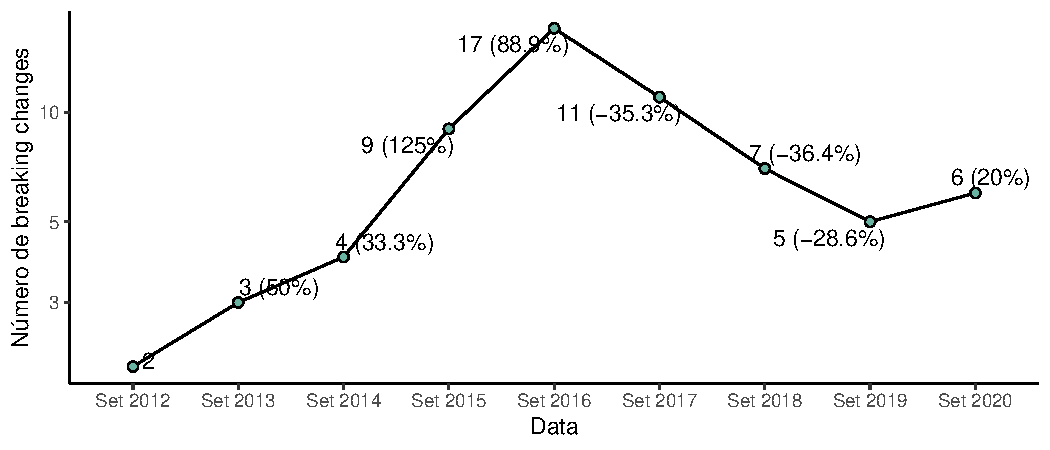
\includegraphics[scale=0.7]{figuras/plot_rq1_2.pdf}
	\caption{Número de casos de \textit{breaking changes} ao longo dos anos}
	\label{fig:plot_rq1_2}
\end{figure}{}

Os casos de \textit{breaking changes} estão crescendo ano após ano. Em média, o fenômeno das \textit{breaking changes} teve um crescimento, de Setembro de 2011 até Setembro de 2016 e de Setembro de 2019 até Setembro de 2020, de 63.4\% desde o respectivo ano anterior. A taxa máxima ocorreu de Setembro de 2014 até Setembro de 2015, período no qual as \textit{breaking changes} aumentaram de 4 casos em 2014 para 9 casos em 2015, um aumento de 125\%. Entretanto, a manifestação das \textit{breaking changes} decresceu de Setembro de 2016 para Setembro de 2019. Esse valor pode ser explicado pelos casos em que não foi possível identificar qual pacote introduziu o erro e, por isso, foram classificados como \textit{Erros não identificados}. Desses casos não identificados, 33.8\% são datados nesse período. Finalmente, a manifestação de \textit{breaking changes} voltou a crescer a partir de Setembro de 2019 de 5 para 6 casos, na taxa de 20\%. Esse é um importante crescimento, considerando que o último pacote cliente da base de dados foi publicado em 1 de Abril de 2020, mas as \textit{breaking changes} continuaram a ser detectadas além de Abril de 2020 devido ao \textit{range} de versões dos provedores.

\subsubsection{Descoberta \#4: 54.9\% das \textit{releases} dos provedores com \textit{breaking changes} possuem mais \textit{commits} do que as outras \textit{releases} no mesmo nível \textit{major}}

As \textit{releases} dos provedores com \textit{breaking changes} possuem uma característica interessante: mais da metade delas possuem mais \textit{commits} do que a mediana dos \textit{commits} em outras \textit{releases} que não introduziram \textit{breaking changes} no mesmo nível \textit{major} do respectivo provedor. Ou seja, foi detectado que, no mesmo nível \textit{major}, o provedor introduz mais \textit{commits} na \textit{release} que introduz uma \textit{breaking change} do que nas \textit{releases} que não introduzem \textit{breaking changes}. Ainda, 42.3\% dessas \textit{releases} possui mais de 50\% de \textit{commits} do que a mediana das demais \textit{releases} no mesmo nível \textit{major}. Ou seja, a cada dois \textit{commit} em uma \textit{release} que não possui \textit{breaking change}, há três \textit{commits} na \textit{release} que introduz \textit{breaking changes}. Esses dados indicam que quando os provedores introduzem mais \textit{commits} do que o usual, eles podem perder o controle das alterações e introduzir mais alterações do que as presumidas pelos clientes. Nesses casos, as alterações introduzidas em uma \textit{release} deveriam ser segmentadas em duas \textit{releases} para haver mais controle das alterações.

Do outro lado, aproximadamente um terço das \textit{releases} dos provedores com \textit{breaking changes} (29.2\%) possuem menos \textit{commits} do que a mediana das outras \textit{releases} no mesmo nível \textit{major}. Dessas \textit{releases}, 57.1\% introduziram apenas um \textit{commit} na \textit{release} e foi esse o \textit{commit} que introduziu a \textit{breaking change}.

\begin{mdframed}
Destaques da QP1: 11.7\% dos pacotes clientes e 13.9\% das \textit{releases} foram impactados por \textit{breaking changes}. O fenômeno das \textit{breaking changes} está frequentemente encerrando a execução dos clientes e tende a crescer 63.4\% a cada ano. Mais da metade das \textit{releases} do provedor que introduzem \textit{breaking changes} recebem mais \textit{commits} do que as outras \textit{releases} no mesmo nível \textit{major}.
\end{mdframed}

%---------------------------------------------------%
%----------------------RQ2--------------------------%
%---------------------------------------------------%

\section{QP2: Erros introduzidos pelos provedores}
\label{sec:qp2:results}

Nesta Seção, estão os resultados e a análise dos dados relacionados à segunda questão de pesquisa: ``Como os pacotes provedores introduzem \textit{breaking changes} em uma \textit{release}?''.

\subsubsection{Descoberta \#5: Categorias de \textit{Breaking changes}}

Ao todo, foram descobertos 64 casos de \textit{breaking changes} distribuídas em 45 clientes. Todos esses casos foram agrupados em 8 categorias das quais se combinavam os casos semelhantes. A Tabela \ref{tab:bc_category} apresenta cada uma dessas categorias, bem como a quantidade de pacotes e a quantidade de \textit{releases} que cada categoria impactou.

\begin{table*}\centering
	\begin{tabular}{lrrrrr} \toprule
		\textbf{Categoria} & \multicolumn{2}{c}{\textbf{Casos}} & \phantom{ab} & \multicolumn{2}{c}{\textit{\textbf{Releases}}}
		\\
		\cmidrule{2-3} \cmidrule{5-6}
		& (\#) & (\%) && (\#) & (\%) \\ \midrule
		Alteração de funcionalidade  & 25              & 39,06 && 101                         & 22,44 \\
		Provedores incompatíveis     & 15              & 23,44 && 64                          & 14,22 \\
		Alteração de tipo de objeto  & 9               & 14,06 && 213                         & 47,33 \\
		Objeto indefinido            & 5               & 7,81  && 28                          & 6,22 \\
		Código incorreto             & 5               & 7,81  && 14                          & 3,11  \\
		Código desatualizado         & 2               & 3,13  && 24                          & 5,33 \\
		Renomeação de função         & 2               & 3,13  && 2                           & 0,44  \\
		Arquivo não encontrado       & 1               & 1,56  && 4                           & 0,89  \\ \hline
		\textbf{Total}               & \textbf{64}     &       && \textbf{450}              &       \\
		\bottomrule
	\end{tabular}
    \caption{Categorias dos casos de \textit{breaking changes}}
    \label{tab:bc_category}
\end{table*}

A seguir, encontra-se uma descrição sobre cada categoria e um exemplo que foi encontrado na análise manual sobre como os provedores introduziram os erros da categoria.

\begin{itemize}
    \item \textbf{Alteração de funcionalidade}: os casos dessa categoria foram os que mais impactaram os clientes. Essa categoria contém os casos de \textit{breaking change} no qual os provedores possuíam um determinado comportamento, mas alteraram algumas de suas regras/funcionalidades e impactaram os seus clientes. Não foi uma simples alteração no código, mas sim uma alteração em regras no qual os clientes tinham como sólida. Por exemplo, a \textit{release} \textsf{request@2.17.0} -- essa \textit{release} foi removida do \textsf{npm}, mas a alteração se manteve -- introduziu uma alteração no código,\footnote{https://github.com/request/request/commit/d05b6ba} como pode ser visto no Código \ref{diff:bc_category_change_rule_1}.
    \vspace{0.4cm}
    \begin{lstlisting}[numbers=none, language=diff, label=diff:bc_category_change_rule_1, caption={Exemplo da categoria \textit{Alteração de funcionalidade}}]
  debug('emitting complete', self.uri.href)
+ if(response.body == undefined && !self._json) {
+   response.body = "";
+ }
  self.emit('complete', response, response.body)
    \end{lstlisting}

    Nesse caso, o \textsf{request} adiciona uma \textit{string} vazia ao invés de manter \textit{undefined} no corpo de uma requisição. Esse caso do \textsf{request} ocorreu porque os pacotes provedores evoluem independentemente dos clientes \cite{Foo:2018:ESC:3236024.3275535}. Essa alteração na regra do \textsf{request} reflete em uma evolução do pacote, mas os clientes não esperavam essa alteração e confiavam que o corpo da resposta fosse retornado como \textit{undefined}, por isso os clientes sofreram um erro.

    \item \textbf{Provedores incompatíveis}: nessa categoria, há um provedor direto \textsf{A} e um provedor indireto \textsf{B} envolvido, o qual alterou o seu código, o que não gerou um erro, mas provocou um comportamento inesperado no provedor \textsf{A}. Ou seja, o provedor \textsf{B} passou a ser incompatível com o provedor \textsf{A}. Nessa categoria, nenhum dos provedores contém um erro, mas sim uma incompatibilidade. Um exemplo disso ocorreu com os pacotes \textsf{babel-eslint} e \textsf{escope}, sendo o pacote \textsf{escope} é um provedor indireto do \textsf{babel-eslint}.
    \vspace{0.4cm}
    \begin{lstlisting}[numbers=none, language=diff, label=cod:bc_category_incompatibles_providers, caption={Exemplo da categoria \textit{Provedores incompatíveis}}]
  }
-   },
-   visitClass: {
+ }, {
+   key: 'visitClass',
        value: function visitClass(node) {
    \end{lstlisting}

    A \textit{release} \textsf{escope@3.4} realizou uma alteração no seu código, conforme o Código \ref{cod:bc_category_incompatibles_providers}, mas que não reflete em um erro. Essa alteração impactou diretamente o pacote \textsf{babel-eslint}, mesmo o pacote \textsf{escope} não sendo um provedor direto do \textsf{babel-eslint} e não ter introduzido um erro.\footnote{https://github.com/estools/escope/issues/99\#issuecomment-178151491} Com isso, houve uma incompatibilidade entre os provedores e essa incompatibilidade precisou ser corrigida pelo \textsf{babel-eslint}. Essa \textit{breaking change} durou apenas um dia, mas durante esse período o \textsf{babel-eslint} foi descarregado \textit{80k} vezes do \textsf{npm}.

    \item \textbf{Alteração de tipo de objeto}: em linguagens fortemente tipadas essa categoria de \textit{breaking change} não ocorre, mas no \textsf{Javascript} representam um tipo de \textit{breaking change} que, por muitas vezes, pode nem se manifestar no cliente. Neste trabalho, foram detectados 9 casos (14.06\%) nos quais os provedores alteraram o tipo de algum objeto.
    \vspace{0.4cm}
    \begin{lstlisting}[numbers=none, language=diff, label=cod:bc_category_change_type, caption={Exemplo da categoria \textit{Alteração de tipo de objeto}}]
- this.sockets = [];
+ this.sockets = {};
  this.nsps = {};
    this.connect Buffer = [];
  }
  var socket = nsp.add(this, function() {
-   self.sockets.push(socket);
+   self.sockets[socket.id] = socket;
    self.nsps[nsp.name] = socket;
    \end{lstlisting}

    No Código \ref{cod:bc_category_change_type} o provedor \textsf{socket.io} alterou um \textit{array} para \textit{object}.\footnote{https://github.com/socketio/socket.io/commit/b73d9be} Anteriormente, os clientes iteravam nesse \textit{array}, mas após essa alteração os clientes foram impactados por uma \textit{breaking change}. Mesmo sendo uma simples alteração, muitos clientes do \textsf{socket.io} foram impactados, até mesmo o pacote \textsf{karma},\footnote{https://github.com/socketio/socket.io/issues/2368} um utilitário para testes em \textit{browsers}, que foi forçado a alterar seu código\footnote{https://github.com/karma-runner/karma/commit/3ab78d6} e publicar a \textit{relese} \textsf{karma@0.13.19}. Enquanto essa \textit{breaking change} permaneceu por apenas um dia, o \textsf{karma} recebeu \textit{146k downloads} do \textsf{npm}.

    \item \textbf{Objeto indefinido}: por vezes, os códigos podem estar todos corretos, mas os provedores tentam acessar uma variável que não existe. Esta categoria de \textit{breaking change} representa os casos no qual os provedores tentaram obter acesso à alguma variável/objeto, mas que não existiam.
    \vspace{0.4cm}
    \begin{lstlisting}[numbers=none, language=diff, label=cod:bc_category_undefined_object, caption={Exemplo da categoria de \textit{Objeto Indefinido}}]
+ app.options = app.options || {};
  app.options.babel = app.options.babel || {};
  app.options.babel.plugins = app.options.babel.plugins || [];
    \end{lstlisting}

    Esse tipo de erro surgiu na \textit{release} \textsf{ember-cli-htmlbars-inline-precompile@0.1.3}, na qual o desenvolvedor tenta acessar uma variável que não estava disponível. Mas, assim como o desenvolvedor já havia feito com as demais variáveis do Código \ref{cod:bc_category_undefined_object}, uma simples alteração no código\footnote{https://github.com/ember-cli/ember-cli-htmlbars-inline-precompile/pull/5/commits/b3faf959} foi o suficiente.

    \item \textbf{Código incorreto}: este caso de \textit{breaking change} ocorreu quando os provedores escrevem um código semanticamente incorreto, gerando um erro na sua execução e afetando os clientes. Em linguagens compiladas, esse tipo de erro seria facilmente identificado em tempo de compilação, mas no \textsf{Javascript} esse tipo de erro apenas se manifesta em tempo de execução. Foi o que ocorreu com a \textit{release} \textsf{front-matter@0.2.0}.
    \vspace{0.4cm}
	 \begin{lstlisting}[numbers=none, language=diff, label=cod:bc_category_wrong_code, caption={Exemplo da categoria \textit{Código incorreto}}]
  const separators = [ '---', '= yaml =']
- const pattern = pattern = '^('
+ const pattern = '^('
    + '((= yaml =)|(---))'
	 \end{lstlisting}

    Apesar de ser um erro facilmente detectável e corrigível, como o provedor fez\footnote{https://github.com/jxson/front-matter/commit/f16fc01} no Código \ref{cod:bc_category_wrong_code}, o provedor \textsf{front-matter} aguardou aproximadamente um ano para corrigir e publicar a \textit{release} \textsf{front-matter@0.2.2}. Durante esse período, \textsf{front-matter} foi descarregado do \textsf{npm} 366 vezes.

    \item \textbf{Código desatualizado}: nessa categoria um provedor \textsf{A} atualiza o seu provedor \textsf{B} explicitamente -- alterando manualmente o \textit{range} do seu provedor no \textit{package.json} --, mas o provedor \textsf{A} não atualiza o seu código para executar de acordo com a nova versão do provedor \textsf{B}. Consequentemente, uma \textit{breaking change} é introduzida nos pacotes clientes. Além de um caso de atualização explícita, foi detectado um caso no qual um provedor \textsf{A} especificou um provedor \textsf{B} com o \textit{X-range ($>$=)}, e ao longo do tempo o provedor \textsf{B} publicou uma \textit{release major} que introduziu \textit{breaking changes}. Apesar do provedor \textsf{A} especificar um \textit{X-range}, \textsf{A} não atentou-se para a atualização implícita de \textsf{B} com uma \textit{breaking change}, e essa \textit{breaking change} foi cascateada para os clientes.

    \item \textbf{Renomeação de função}: as \textit{breaking changes} relacionadas à esta categoria são facilmente detectáveis. Quando a mensagem de erro do \textsf{Node.js} é exibida como \textit{TypeError: var is not a function}, provavelmente trata-se de uma determinada função que não esta disponível, ou seja, foi removida ou renomeada. Todas os dois casos nesta categoria ocorreram porque a função foi renomeada. O primeiro caso está descrito nos exemplos motivacionais (Capítulo \ref{cap:exemplos}).
    \vspace{0.4cm}
	 \begin{lstlisting}[numbers=none, language=diff, label=cod:bc_category_renamed_function, caption={Exemplo da categoria \textit{Renomeação de função}}]
- RedisClient.prototype.send_command = function (command, args, callback) {
-     var args_copy, arg, prefix_keys;
+ RedisClient.prototype.internal_send_command = function (command, args, callback) {
+     var arg, prefix_keys;
	 \end{lstlisting}

    O segundo caso ocorreu quando a \textit{release} \textsf{redis@2.6.0-1} renomeou uma função, como no Código \ref{cod:bc_category_renamed_function}.\footnote{https://github.com/NodeRedis/node\_redis/commit/861749f} Entretanto, essa função era apenas utilizada internamente pelo pacote \textsf{fakeredis},\footnote{https://github.com/NodeRedis/node-redis/issues/1030\#issuecomment-205379483} que foi impactado pela \textit{breaking change}. Essa \textit{breaking change} foi corrigida no pacote cliente \textsf{fakeredis@1.0.3} que realizou um \textit{downgrade} para a versão \textsf{redis@2.6.0-0}.\footnote{https://github.com/hdachev/fakeredis/commit/01d1e99} Em cinco dias nos quais a \textit{breaking change} não foi corrigida, o \textsf{fakeredis} foi descarregado \textit{2.3k} vezes do \textsf{npm}.

    \item \textbf{Arquivo não encontrado}: os casos de \textit{breaking change} relacionados à esta categoria são aqueles no qual os desenvolvedores realizam um acesso a um arquivo que não existe. O arquivo requerido pode não existir ou não estar disponível, uma vez que, referenciado no arquivo \textit{.npmignore} -- arquivo utilizado pelo \textsf{npm} para ignorar arquivos durante o processo de publicação --, o arquivo existe mas não está disponível. Entretanto, o único caso de \textit{breaking change} dessa categoria ocorreu pois o provedor referenciou o \textit{index.js} ao \textit{.npmignore}.
\end{itemize}{}

\subsubsection{Descoberta \#6: Nível do Versionamento Semântico que as \textit{breaking changes} são introduzidas}

De todos os 64 casos de \textit{breaking changes}, 3 casos foram introduzidos no nível \textit{major}; 26 casos, no \textit{minor}; 28 casos, no \textit{patch}; e 5 casos, pré-\textit{releases}, como pode ser visto na Tabela \ref{tab:semver_levels}. Foram analisados apenas os casos de \textit{breaking changes} em \textit{releases minor} e \textit{patch}, mas houve 3 casos em que a \textit{breaking change} foi introduzida em uma \textit{release major}: em dois casos os provedores escreveram códigos errôneos na \textit{release major} e o cliente a estava usando -- como no caso do \textsf{jsdom@16} (Cap. \ref{cap:exemplos}) -- e o terceiro caso ocorreu quando um provedor \textsf{A}, que depende de um provedor \textsf{B}, aceitou a \textit{release} com \textit{breaking change} através do \textit{X-range ($>$=)} do provedor \textsf{B}, mas não tratou essa \textit{breaking change}.

\begin{table}
	\centering
	\caption{\textit{Breaking changes} por nível do Versionamento Semântico}
	\begin{tabular}{lrr}
		\toprule
		\textbf{Níveis} & \textbf{(\#)} & \textbf{(\%)} \\ \hline
		\textit{Major}       & 03       & 4.69          \\
		\textit{Minor}       & 28       & 43.75         \\
		\textit{Patch}       & 28       & 43.75         \\
		Pré\textit{-release} & 05       & 7.8           \\ \bottomrule
	\end{tabular}
	\label{tab:semver_levels}
\end{table}

Pré-\textit{releases} antecedem suas \textit{releases} estáveis, mas não são consideradas estáveis; qualquer alteração não-retro compatível deve ser resolvida até a versão estável ser publicada.\footnote{https://semver.org/\#spec-item-9} Foram detectadas \textit{breaking changes} em 5 casos de pré-\textit{releases}, mas esses provedores cascatearam essas \textit{breaking changes} para as \textit{releases} estáveis. Por exemplo, a pré-\textit{release} \textsf{redis@2.6.0-1}, descrita na categoria \textit{Renomeação de função} da Seção \ref{sec:qp2:results}, alterou o nome de uma função, e essa alteração não-retro compatível deveria ser corrigida até a \textit{release} estável \textsf{redis@2.6.0}, mas essa alteração foi propagada para a \textit{release} estável, impactando e execução do cliente com uma \textit{breaking change}. Esse exemplo mostra como os provedores não estão devidamente orientados sobre as regras do Versionamento Semântico.

\subsubsection{Descoberta \#7: Provedores introduzem a mesma quantidade de \textit{breaking changes} em \textit{releases minor} e \textit{patch}}

Os provedores introduzem \textit{breaking changes} em níveis não-\textit{major} em dois cenários: 1) em \textit{releases minor}, quando os provedores tinha a intenção de publicar novas funcionalidades retro-compatíveis, mas essas funcionalidades tornaram-se \textit{breaking changes}; e 2) em \textit{releases patch}, quando os provedores tinha o propósito de publicar correções de erros. Nos casos das \textit{releases patch}, os provedores estavam realmente tentando publicar uma correção de erro, mas essas alterações podem não ter consertado o erro anterior, mas sim introduzido mais erros. Para casos em \textit{releases minor}, essas novas funcionalidades podem ser casos reais de \textit{breaking changes} dos quais os provedores têm a responsabilidade de corrigir, ou podem ser novas funcionalidades que os clientes precisam se adaptar. Para analisar esse impasse, foi observado qual pacote corrigiu a \textit{breaking change} e para qual nível a nova \textit{release} foi publicada. A Figura \ref{fig:semver_fixed} apresenta esses dados.

\begin{figure}
	\centering
	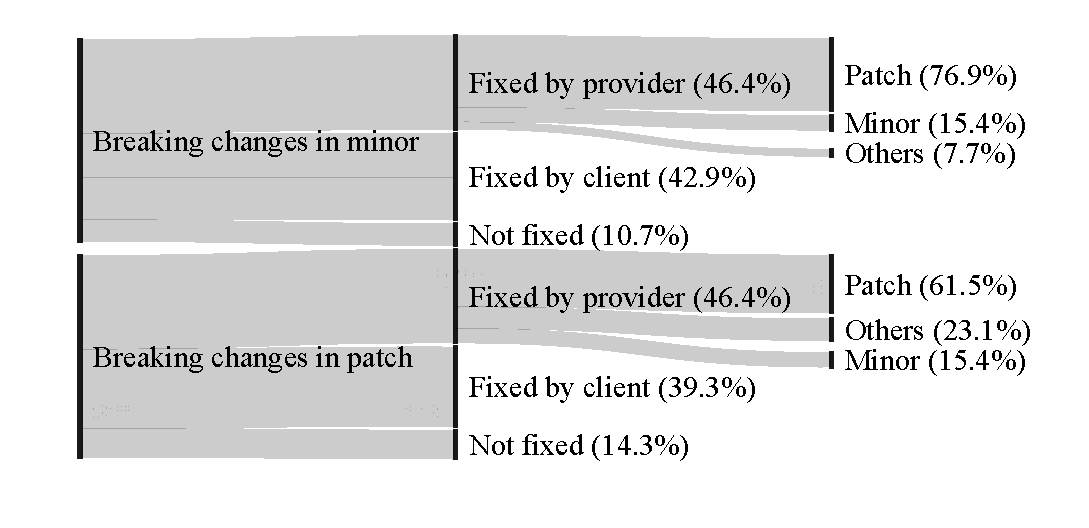
\includegraphics[scale=0.8]{figuras/semver_fixed_prov.pdf}
	\caption{As \textit{breaking changes} corrigidas pelos pacotes providores e clientes e o respectivo nível do Versionamento Semântico que a \textit{release} de correção foi publicada}
	\label{fig:semver_fixed}
\end{figure}{}

A Figura \ref{fig:semver_fixed} mostra que metade das \textit{breaking changes} introduzidas em \textit{releases minor} são corrigidas pelos pacotes clientes. Ou seja, os provedores introduziram uma funcionalidade retro-compatível que tornou-se uma \textit{breaking change}, mas foram os pacotes clientes quem precisaram se adaptar. Mas, quando os provedores corrigem as \textit{breaking changes} introduzidas em \textit{releases minor}, em 76.9\% dos casos a correção é publicada em uma \textit{release patch} e, de acordo com o Versionamento Semântico, essa \textit{release} tinha a finalidade de corrigir um erro. Portanto, os provedores assumem que, de fato, uma \textit{breaking change} foi introduzida e são eles os responsáveis pela correção.

\textit{Breaking changes} introduzidas em \textit{releases patch} deveriam conter apenas correções de erros, mas os provedores introduziram \textit{breaking changes}. Essas \textit{breaking changes} em \textit{releases patch} são corrigidas pelos provedores em 46.4\% das vezes. Ainda, em 61.5\% das vezes os provedores publicam a correção em uma \textit{release patch}, significando que houve a tentativa de corrigir algo.

\subsubsection{Descoberta \#8: 78.1\% das \textit{breaking changes} possuem pelo menos uma documentação}

Quando uma \textit{breaking change} se manifesta nos pacotes clientes, ela deve ser documentada em \textit{issues} ou \textit{pull-requests}. Essas funcionalidades integradas aos repositórios dos pacotes permitem aos clientes notificarem os provedores sobre erros ou questões acerca do próprio provedor. Também, as \textit{breaking changes} podem ser documentadas em \textit{changelogs}, tanto quando a \textit{breaking change} é introduzida ou quando a mesma é corrigida. As \textit{changelogs} criadas pelos provedores contêm os detalhes das alterações que os provedores introduzem em uma determinada \textit{release}.

\begin{table}
	\centering
	\caption{Como cada \textit{breaking change} foi documentada}
	\begin{tabular}{lrr}
		\toprule
		\textbf{Documentação} & \textbf{(\#)} & \textbf{(\%)}   \\ \hline
		\textit{Issue}        & 32            & 64              \\
		\textit{Pull-request} & 22            & 44              \\
		\textit{Changelog} de introdução & 23 & 46              \\
		\textit{Changelog} de correção   & 16 & 32              \\ %\midrule
		%\textbf{Total}         & \textbf{50} & \textbf{78.1\%} \\ 
		\bottomrule
	\end{tabular}
	\label{tab:bc_documentation}
\end{table}

A Tabela \ref{tab:bc_documentation} mostra que as \textit{breaking changes} são documentadas em 55 casos (78.1\%). Dos casos documentados, 70\% possuem mais de um tipo de documentação. Por exemplo, o provedor foi notificado de uma \textit{breaking change} através de uma \textit{issue}, corrigiu-a e a documentou em seu \textit{changelog}. Nesse caso houveram duas documentações. Esse é um número positivo para os clientes, uma vez que quando a mesma \textit{breaking change} se manifesta em vários clientes, mas já foi previamente documentada, torna-se fácil para os clientes se recuperarem. Por fim, em 14 casos (21.9\%) a \textit{breaking change} não foi documentada.

\begin{mdframed}
Destaques da QP2: Os defeitos mais comuns nos pacotes provedores que causam \textit{breaking changes} são aqueles relacionados com uma alteração de funcionalidade, quando dois provedores se tornam incompatíveis e alterações nos tipos de objetos. Os provedores introduzem \textit{breaking changes} em níveis \textit{minor} e \textit{patch} na mesma frequência. A maioria das \textit{breaking changes} corrigidas pelos provedores são publicada em \textit{releases patch}. As \textit{breaking changes} são documentadas em 78.1\% dos casos e a principal funcionalidade usada para documentação são as \textit{issues}.
\end{mdframed}

%---------------------------------------------------%
%----------------------RQ3--------------------------%
%---------------------------------------------------%

\section{QP3: Recuperação dos clientes}
\label{sec:qp3:results}

Esta Seção apresenta os resultados da terceira questão de pesquisa: ``Como os pacotes clientes se recuperam das \textit{breaking changes}?''.

\subsubsection{Descoberta \#9: A maioria das \textit{breaking changes} são introduzidas pelos provedores indiretos}

As \textit{breaking changes} também podem ser introduzidas pelos provedores indiretos e propagadas para os clientes. A Tabela \ref{tab:dependency_tree_deep} apresenta a profundidade/nível da árvore de dependência do cliente em que os provedores que introduziram as \textit{breaking changes} estavam. Apenas 42.2\% das \textit{breaking changes} são introduzidas pelos provedores que o cliente realmente instalou e usa no seu código, ou seja, os provedores diretos que estão referenciados no \textit{package.json} do cliente. Esses provedores estão no primeiro nível da árvore de dependências.

\begin{table}
	\centering
	\caption{O quão profundo os provedores que introduziram a \textit{breaking change} estão do cliente na árvore de dependências}
	\begin{tabular}{lrr}
		\toprule
		\textbf{Nível} & \textbf{(\#)} & \textbf{(\%)} \\ \hline
		1              & 27            & 42.2          \\
		2              & 30            & 46.9          \\
		$>$3           & 07            & 10.9          \\ \bottomrule
	\end{tabular}
	\label{tab:dependency_tree_deep}
\end{table}

Um fato interessante é que as \textit{breaking changes} introduzidas pelos provedores indiretos, aqueles que estão nos níveis dois, três e quatro, representam 57.8\% dos casos. Seis casos estão no terceiro nível e um único caso está no quarto nível. Esses provedores não são instalados pelos clientes, mas eles são descarregados pelo \textsf{npm} quando os provedores diretos são instalado. Nesses casos, a \textit{breaking change} podem ser totalmente desconhecida para os pacotes clientes, uma vez que os clientes podem não ter conhecimento sobre esses provedores indiretos.

\subsubsection{Descoberta \#10: \textit{Breaking changes} que são corrigidas pelos provedores sendo clientes}

Um pacote provedor é um pacote que outros pacotes dependem. Entretanto, quando o provedor possui algum provedor, o primeiro provedor pode ser considerado como um cliente do segundo provedor. Por exemplo, na seguinte árvore de dependências  \texttt{cliente}$\rightarrow$\texttt{prov1}$\rightarrow$\texttt{prov2} -- o \texttt{cliente} seria o pacote cliente que teve seus testes executados neste trabalho -- o \texttt{cliente} tem como seu provedor o pacote \texttt{prov1}, e \texttt{prov1} tem o pacote \texttt{prov2} como seu provedor, que é um provedor indireto do pacote \texttt{cliente}. Então, quando a \textit{breaking change} é introduzida pelo \texttt{prov2} e se manifesta em \texttt{prov1}, o \texttt{prov1} pode ser considerado como um pacote cliente de \texttt{prov2} uma vez que na árvore de dependências o \texttt{prov2} é um provedor direto de \texttt{prov1}. A partir desta perspectiva, os próximos resultados são apresentados considerando o pacote cliente como aqueles que são clientes do pacote que introduziu a \textit{breaking changes} -- exceto nos casos classificados como \textit{Provedores incompatíveis} (Subseção \ref{sec:qp2:results}), porque ambos os provedores devem ser considerados como provedores de \texttt{cliente}.

Nesse contexto, a Tabela \ref{tab:package_fix} apresenta quais pacotes corrigiram cada caso de \textit{breaking change}. A maioria das \textit{breaking changes} foram consertados pelos pacotes provedores. Uma vez que são eles que introduziram a \textit{breaking change}, teoricamente, esse era o comportamento esperado. Os pacotes clientes -- aqueles que tiveram seus testes executados neste trabalho -- recuperaram-se das \textit{breaking changes} em 20.3\% dos casos. Por último, os provedores que são considerados como clientes do provedor que realmente introduziu a \textit{breaking change}, recuperam-se das \textit{breaking changes} em 18.8\% dos casos. Isso é ótima observação para os pacotes clientes, pois os provedores como clientes corrigem as \textit{breaking changes} muitas vezes. Então, quando a \textit{breaking change} não é corrigida pelo provedor que a introduziu, outro provedor, que é o cliente do provedor que introduziu a \textit{breaking change}, pode consertar a \textit{breaking change}.

\begin{table}
	\centering
	\caption{Pacotes que consertaram a \textit{breaking change}}
	\begin{tabular}{lrr}
		\toprule
		\textbf{Consertado por} & \textbf{(\#)} & \textbf{(\%)} \\ \hline
		Provedor                & 32            & 50            \\
		Cliente                 & 13            & 20.3          \\
		Provedor como cliente   & 12            & 18.8          \\
		Não consertado          & 07            & 10.9          \\ \bottomrule
	\end{tabular}
	\label{tab:package_fix}
\end{table}

Entretanto, considerando os cliente e os provedores como clientes, as \textit{breaking changes} são consertadas pelos clientes em 39.1\% dos casos. Esse valor indica que por várias vezes os clientes têm a tarefa de se recuperarem das \textit{breaking changes}.

\subsubsection{Descoberta \#11: Provedores como clientes são os pacotes que corrigem as \textit{breaking changes} mais rapidamente}

Quando uma \textit{breaking change} é introduzida, ela deve ser corrigida pelos provedores que a introduziram, pelos provedores como clientes ou pelos pacotes clientes. A Tabela \ref{tab:fix_day} apresenta o tempo que cada pacote gastou para consertar os casos de \textit{breaking changes}. Em geral, as \textit{breaking changes} são consertadas em 7 dias pelo provedor que as introduziram. Mesmo considerando esse curto período de tempo, um grande número de clientes diretos e indiretos podem ser afetados pelas \textit{breaking change} enquanto elas não são corrigidas.

% \begin{table}
% 	\centering
% 	\caption{Mediana dos dias que cada pacote gastou para consertar os casos de \textit{breaking changes} e o tempo que os clientes e provedores como clientes gastam para realizar um \textit{upgrade}/\textit{downgrade} na versão dos provedores}
% 	\begin{tabular}{lrrrrrr} \toprule
% 		\textbf{Corrigido por} & \textbf{Dias} & \multicolumn{2}{c}{\textbf{Recuperado de}} & \phantom{ab} & \multicolumn{2}{c}{\textbf{Tempo para}}
% 		\\
% 		\cmidrule{3-4} \cmidrule{6-7}
% 		                   &    & implícito   & explicito   && \textit{downg}. & \textit{upgr}.       \\ \midrule
% 		Provedor           & 06 & \textemdash & \textemdash && \textemdash     & \textemdash \\
% 		Cliente            & 34 & 34          & 82          && 18.5            & 78          \\
% 		Prov. como Cliente & 04 & 04          & \textemdash && 125.5           & 04           \\ \hline
% 		\textbf{Total}     & \textbf{07} & \textbf{10.5} & \textbf{82} && \textbf{18.5} & \textbf{10.5} \\
% 		\bottomrule
% 		\label{tab:fix_day}
% 	\end{tabular}
% \end{table}

\begin{table}
	\centering
	\caption{Mediana dos dias gastos para consertar as \textit{breaking changes}}
	\begin{tabular}{lrr}
		\toprule
		\textbf{Consertador por} & \textbf{Dias} \\ \hline
		Provedor                 & 06            \\
		Cliente                  & 34            \\
		Provedor como cliente    & 04            \\
		\textbf{Total}           & 07            \\ \bottomrule
	\end{tabular}
		\label{tab:fix_day}
\end{table}

No geral, os pacotes que mais rápido corrigem as \textit{breaking changes} são os provedores como clientes. Na verdade, a uma \textit{breaking change} somente existe quando ela se manifesta nos pacotes clientes, portanto, os provedores como clientes são os primeiros pacotes a serem afetados pelas \textit{breaking changes} e são os que realmente precisam se recuperar. Considerando os provedores e os provedores como clientes, as \textit{breaking changes} são corrigidas em uma mediana de 5 dias por esses provedores, enquanto que os clientes gastam 34 dias para se recuperarem das \textit{breaking chnages}. Então, os pacotes que devem corrigir as \textit{breaking changes} são os provedores e os provedores como clientes, uma vez que os clientes demoram para se recuperarem e, de acordo com a Tabela \ref{tab:package_fix}, os provedores e os provedores como clientes são os que corrigem a maioria das \textit{breaking change} (78.8\%). Finalmente, as \textit{breaking changes} indiretas -- aquelas corrigidas pelos provedores como clientes -- são consertadas 1.5 vezes mais rápidas do que as \textit{breaking changes} diretas.

\subsubsection{Descoberta \#12: Como os clientes se recuperam das \textit{breaking changes}}

A Tabela \ref{tab:version_change} apresenta os dados sobre as formas que os clientes se recuperam das \textit{breaking changes}. Em 48 casos os clientes alteraram a versão de seus provedores -- mesmo quando os provedores consertam as \textit{breaking changes}. Apesar de ser a maneira mais fácil de se recuperaram das \textit{breaking changes}, na maioria dos casos (71.4\%), ao invés de realizarem um \textit{downgrade}, os pacotes clientes realizam um \textit{upgrade} na versão de seus provedores. A partir desse resultado, foi verificado todos os casos onde os clientes e os provedores como clientes consertaram a \textit{breaking change} apenas alterando a versão do provedor antes do provedor ter consertado a \textit{breaking change}. Foi observado que os clientes e provedores como clientes realizam um \textit{upgrade} em 12 (52.2\%) casos de 23. Ou seja, mais da metade dos casos do qual os clientes e os provedores como clientes consertaram a \textit{breaking change}, os pacotes provedores já tinham \textit{releases} mais atuais mas esses clientes não estavam usando essas novas \textit{releases}.

% \begin{table*}
% 	\centering
% 	\caption{Como os pacotes clientes alteram a versão dos provedores após uma \textit{breaking change}}
% 	\begin{tabular}{lcccccccccccc} \toprule
% 		\textbf{Pacote} & \textbf{Total} & \multicolumn{2}{c}{\textbf{\textit{Upgr.}}} & \phantom{ab} & \multicolumn{2}{c}{\textbf{\textit{Downg.}}} & \phantom{ab} & \multicolumn{2}{c}{\textbf{Troca}} & \phantom{ab} & \multicolumn{2}{c}{\textbf{Remoção}}
% 		\\ \cmidrule{3-4} \cmidrule{6-7} \cmidrule{9-10} \cmidrule{12-13}
% 		                      &    & (\#) & (\%) && (\#) & (\%) && (\#) & (\%) && (\#) & (\%) \\ \midrule
% 		Cliente               & 28 & 20   & 71.4 && 06   & 21.4 && 01   & 3.6  &&  01  & 3.6  \\
% 		Provedor como Cliente & 20 & 09   & 45   && 10   & 50   && 01   & 05   && \textemdash & \textemdash \\ \bottomrule
% 		\label{tab:version_change}
% 	\end{tabular}
% \end{table*}
\vspace{0.4cm}
\begin{table}
	\centering
	\caption{Como os pacotes clientes alteram a versão dos provedores após uma \textit{breaking change}}
	\begin{tabular}{lcccccccc} \toprule
		\textbf{Pacote} & \textbf{Total} & \textbf{\textit{Upgr.}} & \textbf{\textit{Downg.}} & \textbf{Troca} & \textbf{Remoção} \\ \midrule
		Cliente               & 28 & 71.4\% & 21.4\% & 3.6\%  & 3.6\%  \\
		Provedor como Cliente & 20 & 45\%   & 50\%   & 05\%   & \textemdash \\ \bottomrule
		\label{tab:version_change}
	\end{tabular}
\end{table}

O número de \textit{downgrades} nos provedores como clientes pode explicar o motivo pelo qual corrigem as \textit{breaking changes} mais rápido que outros pacotes. Uma vez que os provedores como clientes também são provedores, eles devem consertar as \textit{breaking changes} o mais rápido possível, assim evitando a propagação das \textit{breaking changes}. Portanto, realizar um \textit{downgrade} para uma \textit{release} estável do provedor, como ocorreu na metade dos casos, é a maneira mais rápida de se recuperar das \textit{breaking changes}. Finalmente, em uma pequena proporção, os provedores são removidos ou trocados após a introdução das \textit{breaking changes}. Isso mostra o quão dependente os pacotes cliente podem ser dos seus provedores.

\subsubsection{Descoberta \#13: Os clientes geralmente alteram a versão do provedor, mas para o mesmo \textit{range}}

Geralmente, os clientes alteram a versão de seus provedores. Isso garante que o \textsf{npm} não irá instalar as versões prévias do provedor que são aceitas pelo \textit{range}. Entretanto, quando uma \textit{breaking change} se manifesta, é praticamente obrigatório atualizar a versão do provedor. A Figura \ref{fig:semver_both} apresenta quando os clientes e os provedores como clientes atualizaram a versão dos seus provedores.

\begin {figure} [h!]
   \centering
   \mbox {
        \subfigure[Clientes]{\label{fig:semver_cli} 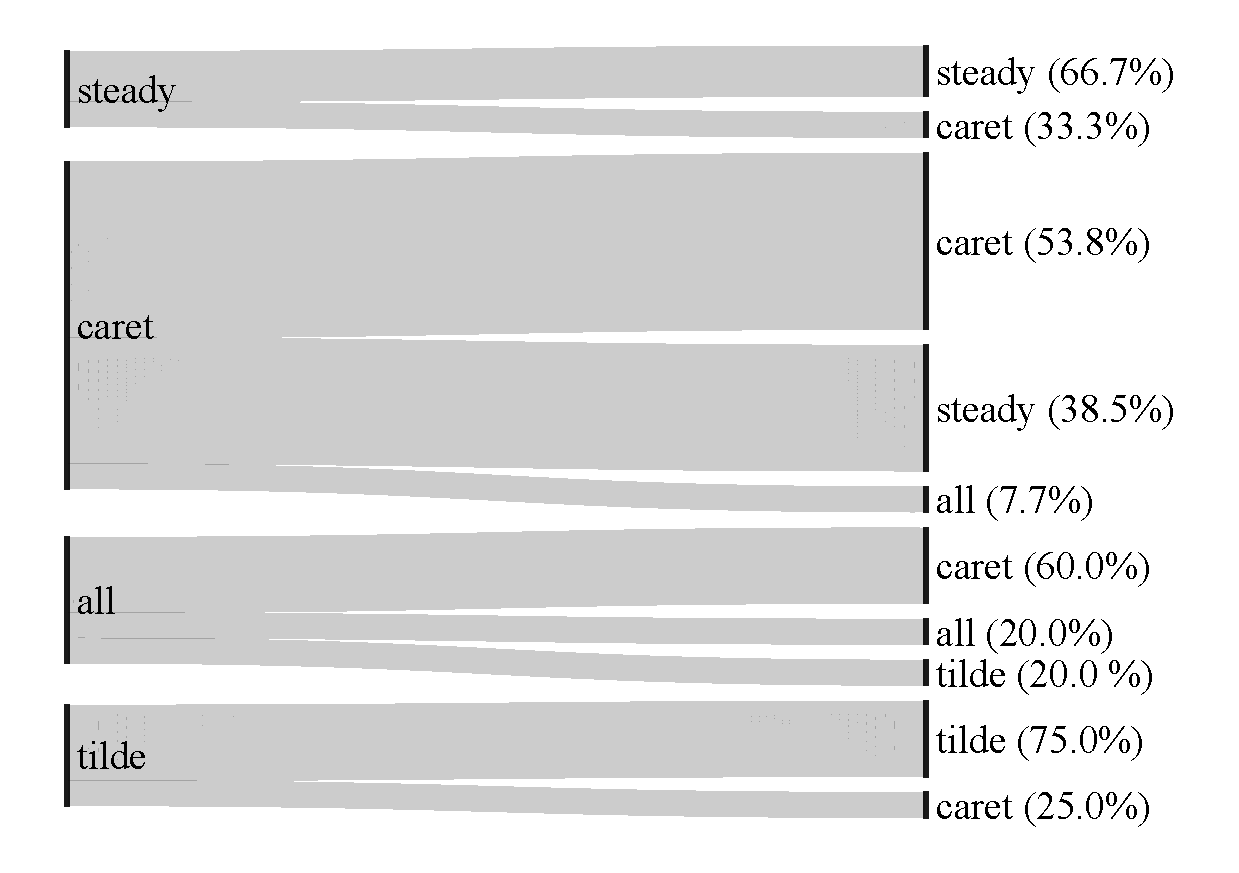
\includegraphics[scale=0.37]{figuras/semver_change_client.pdf}}\quad
        \subfigure[Provedores como clientes]{\label{fig:semver_pac} 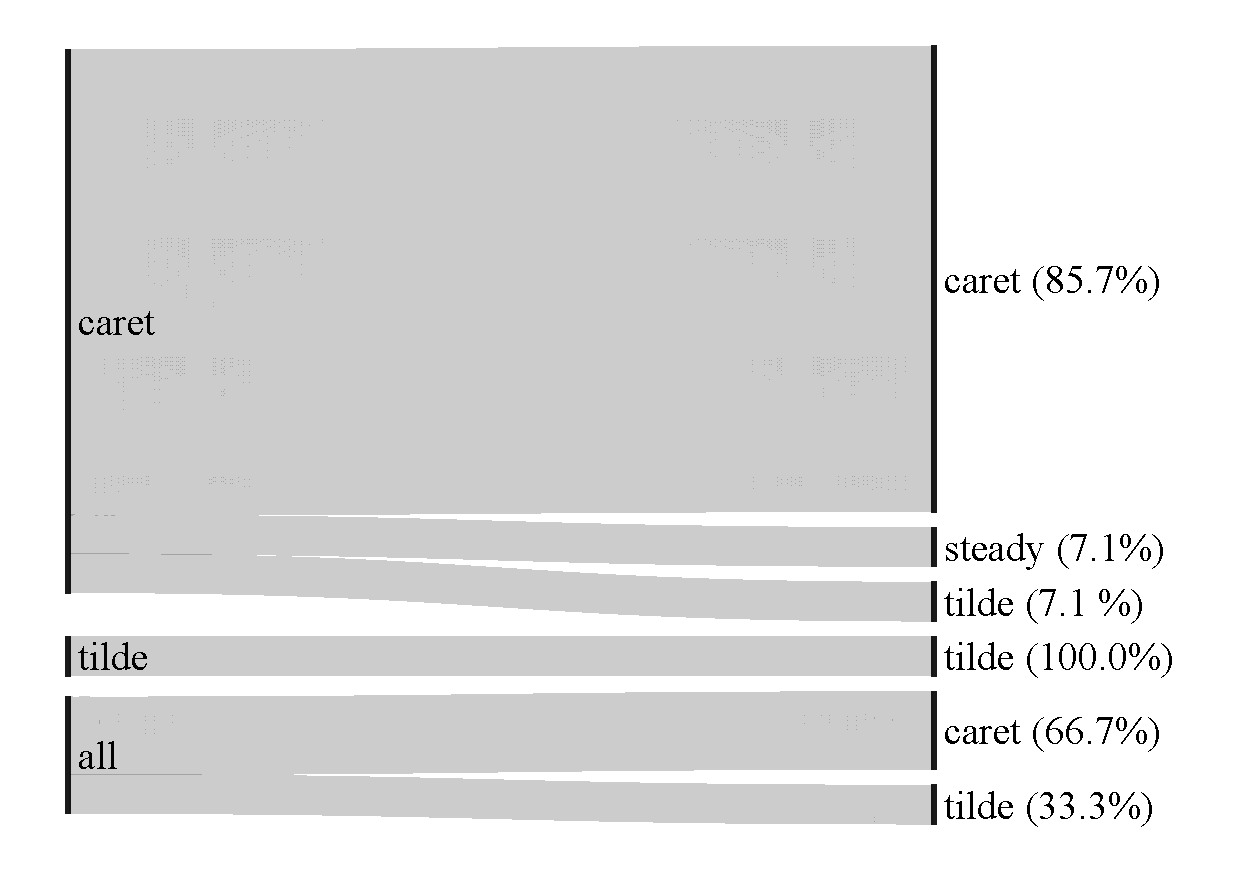
\includegraphics[scale=0.37]{figuras/semver_change_pac.pdf}}
    }
    \caption{A versão dos provedores alteradas pelos clientes e pelos provedores como clientes}
    \label{fig:semver_both}
\end{figure}

Foi verificado que os provedores como clientes nunca utilizam a versão de seus provedores como \textit{steady}, ou seja, sem o \textit{range}. Quando uma \textit{breaking change} é manifestada nos provedores como clientes, eles sempre estão usando os seus provedores com um \textit{range}. Entretanto, apenas em um único caso o provedor como cliente alterou o \textit{range} de um \textit{caret} para um \textit{steady}. Mas, quando os clientes estão usando um \textit{range caret} e são impactados por uma \textit{breaking change}, em 38.5\% dos casos, eles realizam um \textit{downgrade} na versão do provedor alterando para um \textit{range steady}. Essa é a maneira mais rápida e fácil de se recuperar de uma \textit{breaking change}, mas o empecilho está no fato de se utilizar uma versão antiga do provedor.

A maioria das \textit{breaking changes} são introduzidas quando os clientes e provedores como clientes estão usando o \textit{range caret}. Esse é o \textit{range} padrão que o \textsf{npm} insere no \textit{package.json} quando os provedores são instalado. Mais da metade dos casos, esses clientes alteram a versão dos provedores para outro \textit{range caret}. Ainda, os \textit{X-range}, ou \textit{range all}, são os menos usados e os apenas uma minoria das alterações de \textit{range} são convertidas para um \textit{X-range}.

Os clientes e provedores como clientes tendem a manter o mesmo \textit{range}, apenas atualizando esse \textit{range}. Em 60.5\% dos casos, o tipo do \textit{range} (\textit{X-range}, \textit{range caret}, \textit{range tilde} ou \textit{steady}) é mantido, mas é realizado um \textit{downgrade/upgrade} no \textit{range} do provedor. Por exemplo, um cliente especifica o provedor como \textsf{p@\textasciicircum1.2.0} e recebe uma \textit{breaking change} em \textsf{p@1.3.2}. Se o provedor corrige o erro, o cliente irá atualizar para, por exemplo, \textsf{p@\textasciicircum1.4.0}, mas não irá mudar para outro tipo de \textit{range}, tal como para um \textit{range tilde}.

\subsubsection{Descoberta \#14: As \textit{breaking changes} documentadas são corrigidas 3.3 vezes mais rápidas do que as \textit{breaking changes} não documentadas}

\textit{Breaking changes} podem ser documentadas em \textit{issues}, \textit{pull-requests} ou \textit{changelogs}. Tais documentações ocorrem em 78.1\% dos casos. A documentação afeta diretamente o tempo gasto para corrigir uma \textit{breaking change}. As \textit{breaking changes} que possuem pelo menos um tipo de documentação são corrigidas, em mediana, 3 dias após serem introduzidas. Em oposição, quando as \textit{breaking changes} não são documentadas elas recebem uma correção somente após 10 dias. Então, a documentação é muito importante para os clientes e os provedores quando eles estão tentando rastrear e corrigir as \textit{breaking changes}

\begin{mdframed}
Destaques da QP3: Os pacotes clientes, incluindo os clientes diretos e os provedores como clientes, corrigem as \textit{breaking changes} em 39.1\% dos casos. Os casos de \textit{breaking changes} introduzidas pelos provedores indiretos são os mais comuns. Também, os provedores corrigem as \textit{breaking changes} mais rápidos do que os clientes, e os clientes preferem realizar um \textit{upgrade} a um \textit{downgrade} na versão do provedor. Finalmente, o \textit{range} dos provedores podem ser alterados após uma \textit{breaking changes}, mas, no geral, os clientes não alteram o tipo do \textit{range}. As \textit{breaking changes} documentadas são corrigidas 3.3 vezes mais rápido do que as demais.
\end{mdframed}